\chapter{Oscilador Controlado por Tensión (VCO)}
\label{chap:vco}

Este capítulo presenta el diseño y simulación del Oscilador Controlado por Tensión (VCO) del radar FMCW.

\section{Introducción Teórica}

Un Oscilador Controlado por Tensión (VCO, por sus siglas en inglés \textit{Voltage Controlled Oscillator}) es un dispositivo capaz de generar una señal periódica cuya frecuencia de oscilación varía en función de una tensión de control aplicada a su entrada. La relación entre la tensión de control $V_{\text{ctrl}}$ y la frecuencia de salida $f_{\text{out}}$ se denomina función de transferencia o sensibilidad del VCO, y se expresa típicamente en $\text{MHz/V}$.

\subsection{Rol del VCO en el Radar FMCW}

En el sistema radar FMCW, el VCO cumple un rol fundamental: es el encargado de generar la señal de radiofrecuencia (RF) que será transmitida hacia el objetivo. Como se describió en el Capítulo \ref{chap:introduccion}, el principio de funcionamiento del radar FMCW se basa en transmitir una señal cuya frecuencia varía linealmente en el tiempo, conocida como señal \textit{chirp}. Esta señal permite determinar la distancia al objetivo mediante la diferencia de frecuencia entre la señal transmitida y la señal reflejada.

El VCO permite generar la señal chirp de manera sencilla: al aplicar una tensión de control en forma de rampa, la frecuencia de salida del oscilador aumenta (o disminuye) linealmente en el tiempo. La pendiente del barrido de frecuencia $m$ (en $\text{Hz/s}$) determina directamente la resolución en distancia del radar, según la ecuación:

\begin{equation}
\Delta t = \frac{\Delta f}{m}
\end{equation}

\noindent donde $\Delta f$ es la diferencia de frecuencia medida entre la señal transmitida y recibida, y $\Delta t$ es el tiempo de viaje de la señal.

\subsection{Señal de Control: Rampa Diente de Sierra}

La señal de control que se aplica al VCO en un radar FMCW es típicamente una rampa de tensión en forma de diente de sierra, como se ilustra en la Figura \ref{fig:fmcw_sawtooth}. Esta señal presenta las siguientes características:

\begin{itemize}
    \item \textbf{Rampa ascendente lineal:} Durante el período de barrido, la tensión aumenta linealmente desde un valor mínimo $V_{\text{min}}$ hasta un valor máximo $V_{\text{max}}$. Esto produce un incremento lineal de la frecuencia de salida del VCO desde $f_{\text{min}}$ hasta $f_{\text{max}}$.
    
    \item \textbf{Retroceso rápido:} Al finalizar cada período de barrido, la tensión retorna rápidamente al valor inicial, reiniciando el ciclo de modulación.
    
    \item \textbf{Período de modulación:} El tiempo de duración de cada rampa $T_{\text{mod}}$ determina, junto con el ancho de banda de barrido $BW = f_{\text{max}} - f_{\text{min}}$, la pendiente de la modulación:
    \begin{equation}
    m = \frac{BW}{T_{\text{mod}}} = \frac{f_{\text{max}} - f_{\text{min}}}{T_{\text{mod}}}
    \end{equation}
\end{itemize}

Es importante destacar que la función de transferencia de un VCO real no es perfectamente lineal, lo que implica que una rampa de tensión lineal no producirá un barrido de frecuencia perfectamente lineal. Para aplicaciones de mayor precisión, se pueden implementar técnicas de precompensación o linealización de la señal de control. Sin embargo, para este diseño de primer orden, esta no linealidad puede ser tolerada.

\subsection{Especificaciones del VCO para el Diseño}

Para el presente diseño del radar FMCW con frecuencia de operación centrada en $1\,\text{GHz}$, el VCO debe cumplir con los siguientes requerimientos:

\begin{itemize}
    \item \textbf{Rango de frecuencia:} El VCO debe ser capaz de oscilar en un rango que incluya la frecuencia central de $1\,\text{GHz}$. Para este diseño se adoptó un ancho de banda de barrido de $BW = 50\,\text{MHz}$, lo que resulta en una resolución en distancia de $\Delta R = \frac{c}{2 \cdot BW} = \frac{3 \times 10^8}{2 \times 50 \times 10^6} = 3\,\text{m}$.
    
    \item \textbf{Sensibilidad (tuning range):} Debe presentar una sensibilidad adecuada para cubrir el ancho de banda de barrido deseado con el rango de tensiones de control disponible. La señal de control será generada por un conversor digital-analógico (DAC) controlado por un microcontrolador.
    
    \item \textbf{Potencia de salida:} Debe entregar suficiente potencia para alimentar la etapa de amplificación de potencia (PA) subsiguiente.
\end{itemize}

\subsection{Circuito de Referencia Utilizado}

Para el diseño del VCO se tomó como referencia el circuito oscilador Clapp presentado en \cite{rosu_vco}, que se muestra en la Figura \ref{fig:clapp_reference}. El oscilador Clapp es una variación del oscilador Colpitts en configuración colector común, ampliamente utilizado en aplicaciones de alta frecuencia debido a su estabilidad y facilidad de sintonización mediante un varactor.

\begin{figure}[htbp]
\centering
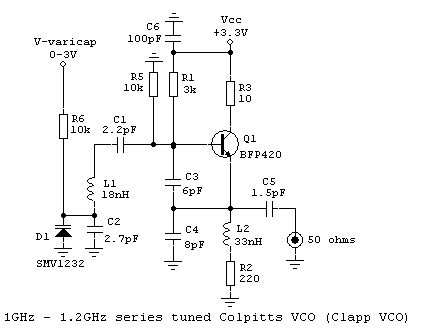
\includegraphics[width=0.7\textwidth]{Figures/3_VCO/Clapp_Reference_Design.png}
\caption{Circuito de referencia del oscilador Clapp \cite{rosu_vco}.}
\label{fig:clapp_reference}
\end{figure}

En este circuito, el transistor $Q1$ en configuración colector común actúa como elemento activo que mantiene la oscilación, mientras que la frecuencia es determinada por los componentes pasivos del circuito tanque resonante. La red de realimentación está formada por los capacitores $C3$ (entre base y emisor) y $C4$ (entre emisor y tierra), que constituyen el divisor capacitivo característico de la topología Colpitts. La red de sintonización consiste en $C1$ en serie con el inductor $L1$, y en paralelo con la combinación del capacitor $C2$ y el diodo varactor $D1$.

La frecuencia de oscilación $f_0$ está determinada por el punto donde la reactancia total del circuito tanque es cero, y viene dada por:

\begin{equation}
f_0 = \frac{1}{2\pi} \sqrt{\frac{1}{L1} \left( \frac{1}{C1} + \frac{1}{C2 + C_{\text{var}}} + \frac{1}{C3} + \frac{1}{C4} \right)}
\label{eq:freq_clapp}
\end{equation}

\noindent donde $C_{\text{var}}$ representa la capacitancia del diodo varactor $D1$, que varía en función de la tensión de control aplicada, permitiendo así el ajuste de la frecuencia de oscilación.

Para que el circuito oscile de manera sostenida, debe cumplir con el criterio de Barkhausen, que establece dos condiciones: la fase total del lazo de realimentación debe ser $0^\circ$ (o múltiplo de $360^\circ$) y la ganancia del lazo $|A\beta|$ debe ser mayor o igual a 1. En la configuración colector común, el transistor no invierte la fase, por lo que la red $LC$ debe presentar fase cero, lo cual ocurre en la frecuencia de resonancia. La condición de ganancia para el arranque se expresa como:

\begin{equation}
g_m \geq R_s \cdot \omega^2 \cdot C3 \cdot C4
\label{eq:condicion_arranque}
\end{equation}

\noindent donde $g_m$ es la transconductancia del transistor y $R_s$ es la resistencia serie parásita del circuito tanque. Esto implica que la corriente de polarización debe ser suficiente para que el transistor compense las pérdidas resistivas del tanque.

\section{Simulación}

\subsection{Diseño del Núcleo del Oscilador}

Para iniciar el diseño en ADS se partió de un diseño existente disponible en la guía de diseño (\textit{DesignGuide}) denominado \textit{Bipolar Modified Clapp Oscillator}, el cual fue posteriormente modificado para adaptarlo a los requerimientos del proyecto. Este diseño presenta una arquitectura modular donde se distinguen claramente dos bloques: el núcleo del oscilador, que contiene el elemento activo y provee la resistencia negativa necesaria para sostener la oscilación, y el resonador, que es la red que determina la frecuencia de resonancia. El varactor se ubica dentro de la estructura del resonador, pero se conecta externamente para facilitar su caracterización.

Esta arquitectura modular ofrece la ventaja de poder configurar los parámetros de forma externa y separar claramente las partes funcionales del oscilador, permitiendo estudiar cada bloque de manera independiente.

El esquemático original fue modificado para aproximarlo al diseño de referencia presentado anteriormente: un oscilador Clapp modificado en configuración colector común. El esquemático y símbolo resultantes se muestran en las Figuras \ref{fig:vco_core_schematic} y \ref{fig:vco_core_symbol}. En este diseño, el componente $C_{\text{cpl}}$ permite ajustar directamente la contribución de la capacitancia del varactor al circuito, controlando así el rango de variación de frecuencia.

\begin{figure}[htbp]
\centering
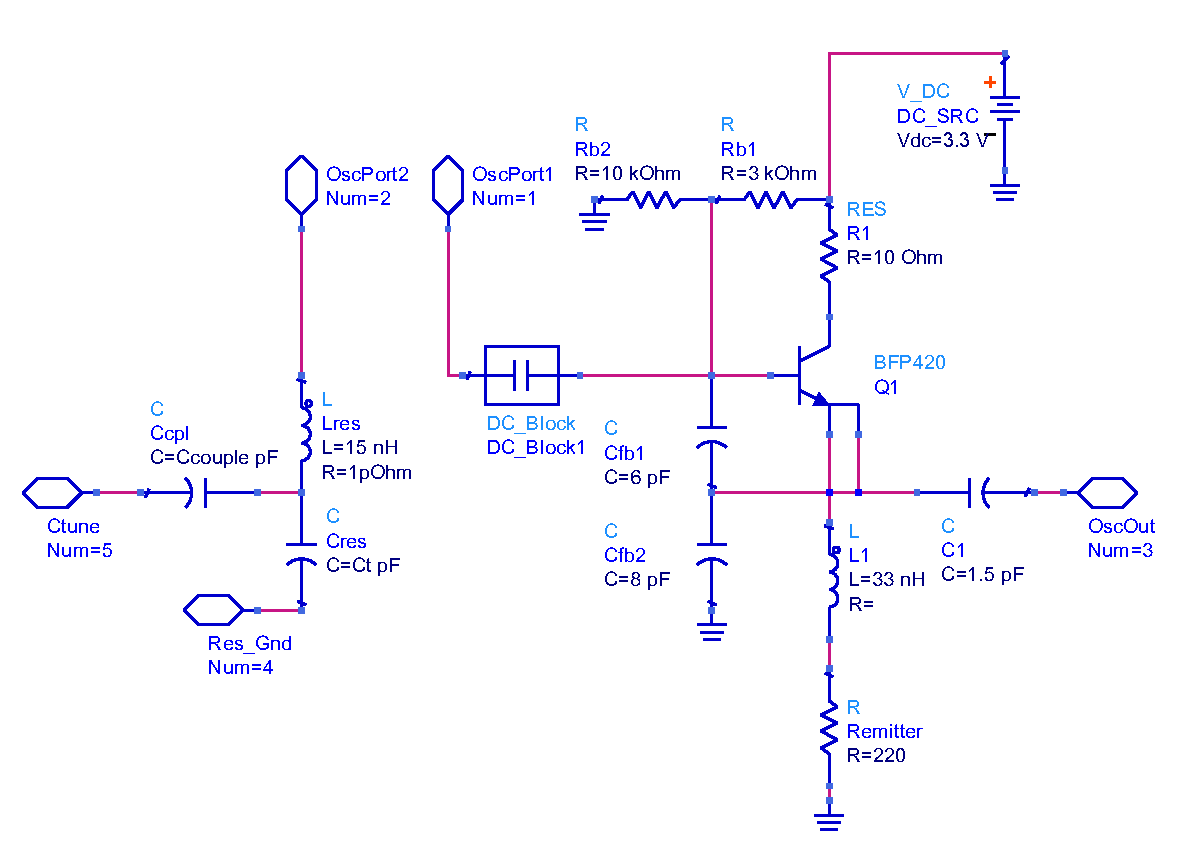
\includegraphics[width=0.8\textwidth]{Figures/3_VCO/vco_core_schematic.pdf}
\caption{Esquemático del núcleo del oscilador Clapp modificado en ADS.}
\label{fig:vco_core_schematic}
\end{figure}

\begin{figure}[htbp]
\centering
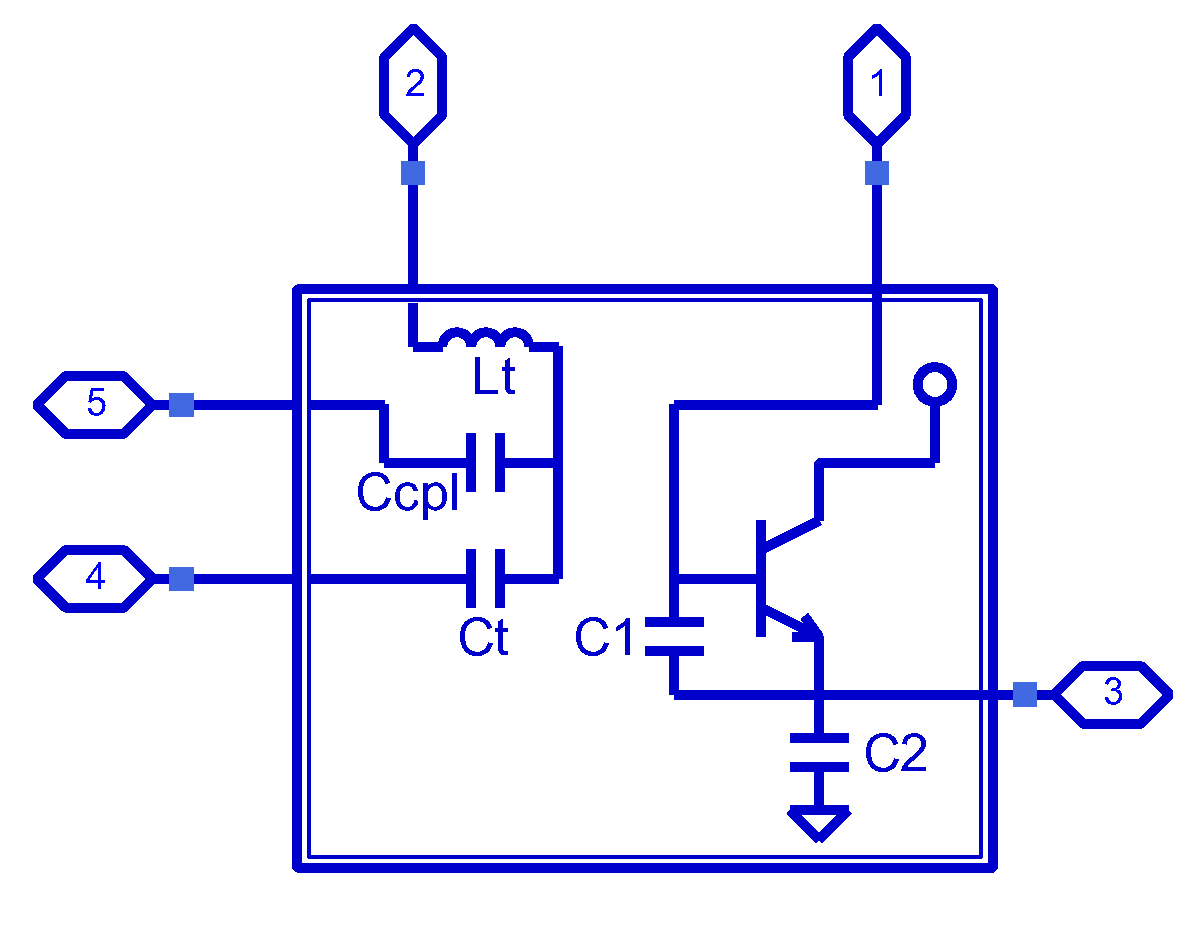
\includegraphics[width=0.4\textwidth]{Figures/3_VCO/vco_core_symbol.pdf}
\caption{Símbolo del núcleo del oscilador en ADS.}
\label{fig:vco_core_symbol}
\end{figure}

Los puertos \texttt{OscPort1} y \texttt{OscPort2} se conectan directamente entre sí durante la operación normal del oscilador. Sin embargo, durante el análisis se inserta una punta de prueba \texttt{OscPort} entre ambos puertos, lo cual habilita al controlador de \textit{Harmonic Balance} para realizar un análisis en modo oscilador.

\subsection{Diseño y Optimización de la Etapa}

En la Figura \ref{fig:vco_optimization_stage} se presenta la configuración final de componentes para la etapa del VCO. Comenzando desde la parte izquierda del esquemático, se tiene la tensión de entrada de control ($V_{\text{tune}}$), una pequeña etapa de amplificación, y el diodo varactor conectados al resonador del componente núcleo del oscilador.

\begin{figure}[htbp]
\centering
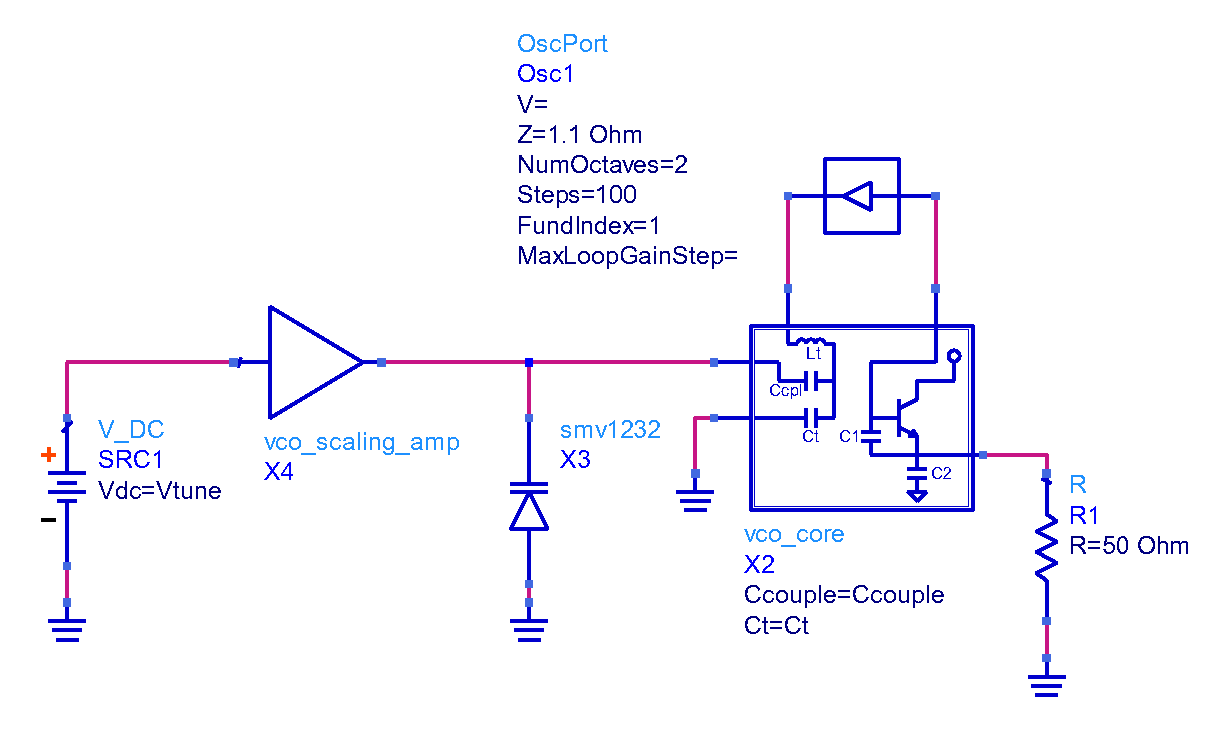
\includegraphics[width=0.95\textwidth]{Figures/3_VCO/vco_optimization_stage.pdf}
\caption{Esquemático de la etapa completa del VCO con varactor y amplificador de escalado.}
\label{fig:vco_optimization_stage}
\end{figure}

La etapa de amplificación provee un ajuste de escala de la señal de control, en caso de que el rango de tensión requerido sea mayor del que puede entregar el dispositivo de control. Se trata de un amplificador operacional en configuración no inversora, basado en el componente LMP7712. En la Figura \ref{fig:vco_scaling_amp} se puede observar el esquemático de esta etapa. Se utilizó el modelo SPICE disponible en el sitio web de Texas Instruments \cite{ti_lmp7712_model} para simular su comportamiento real.

\begin{figure}[htbp]
\centering
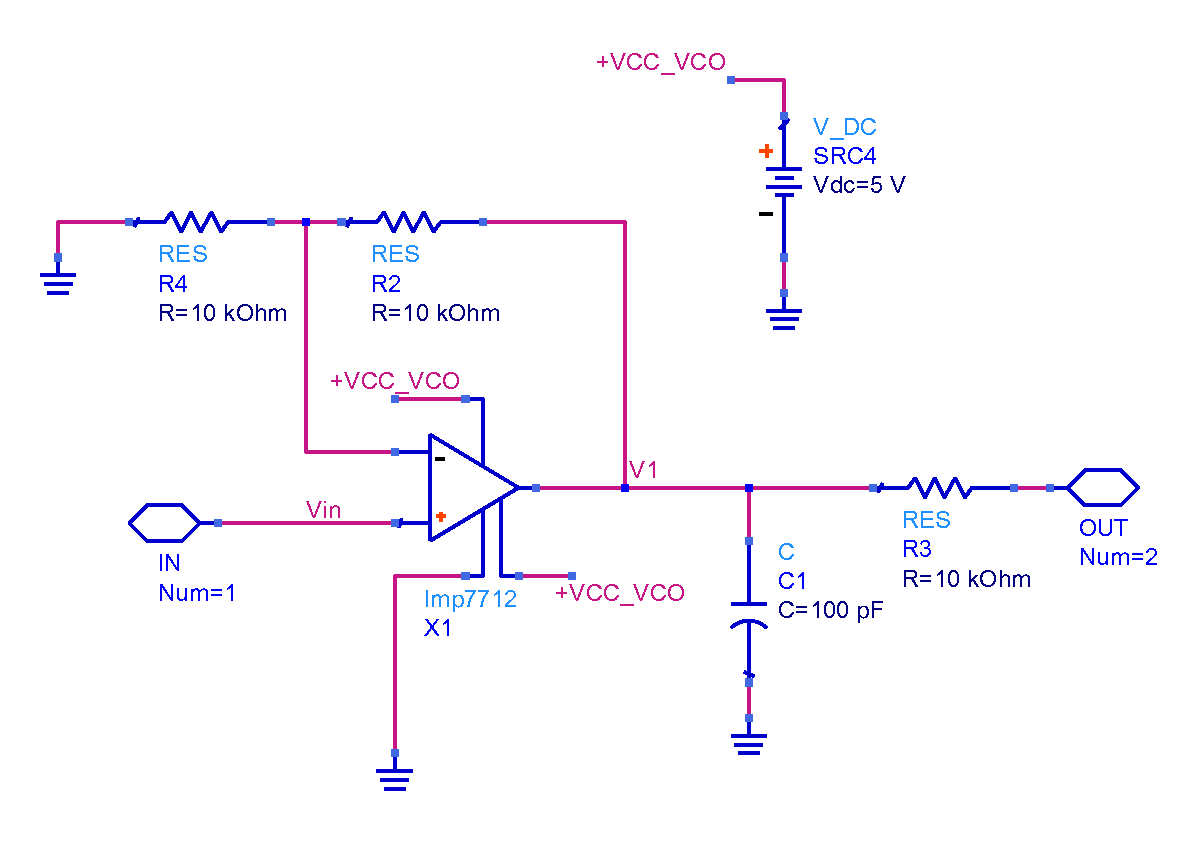
\includegraphics[width=0.8\textwidth]{Figures/3_VCO/vco_scaling_amp.pdf}
\caption{Esquemático del amplificador de escalado basado en LMP7712.}
\label{fig:vco_scaling_amp}
\end{figure}

El diodo varactor seleccionado es el SMV1232 de Skyworks, parte de la serie SMV123x de diodos varactores de silicio de unión hiperabrupta, los cuales están diseñados para su uso en VCOs de alto Q. Para simular el comportamiento de este diodo de la manera más cercana a la realidad, se consultó una nota de aplicación del fabricante \cite{skyworks_varactor_spice}, orientada específicamente a diseños de VCOs, en la cual se propone un modelo equivalente basado en el modelo no lineal de diodo con sus pérdidas representadas por elementos discretos. En la Figura \ref{fig:vco_smv1232} se muestra el esquemático del modelo del varactor, cuyo comportamiento fue verificado mediante un test bench.

\begin{figure}[htbp]
\centering
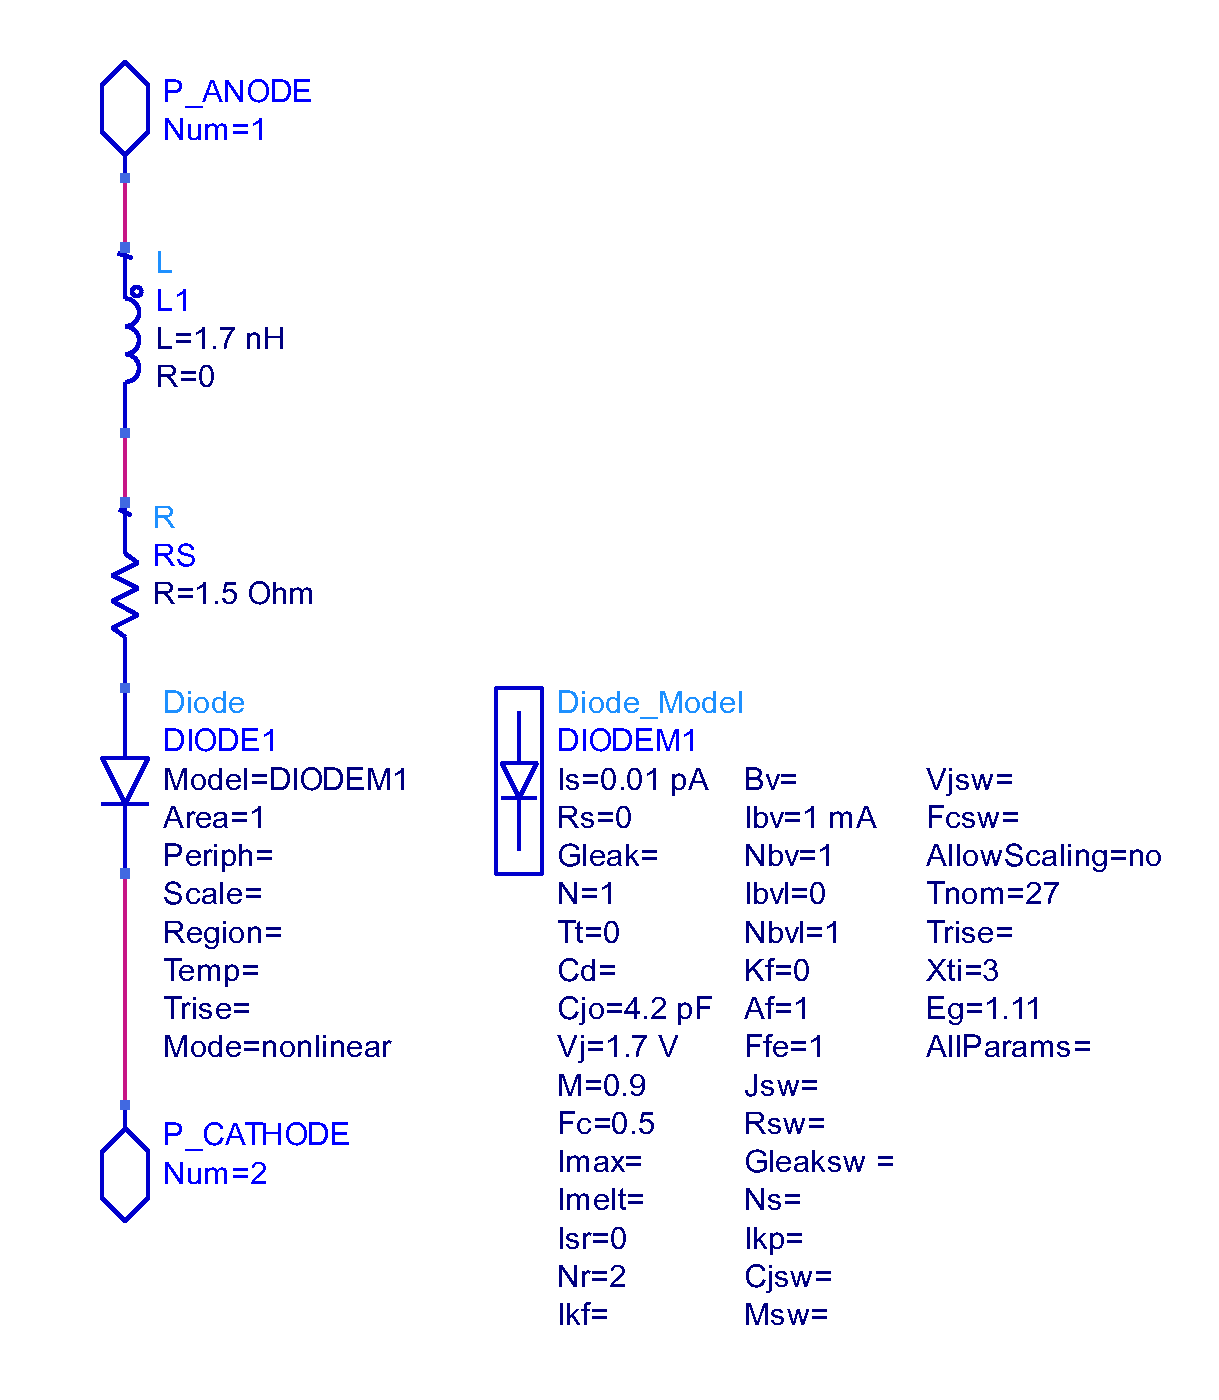
\includegraphics[width=0.6\textwidth]{Figures/3_VCO/vco_smv1232.pdf}
\caption{Modelo SPICE del diodo varactor SMV1232.}
\label{fig:vco_smv1232}
\end{figure}

Los parámetros del modelo SPICE para el SMV1232 se resumen en la Tabla \ref{tab:smv1232_params}.

\begin{table}[htbp]
\centering
\caption{Parámetros del modelo SPICE del varactor SMV1232.}
\label{tab:smv1232_params}
\begin{tabular}{llcl}
\toprule
\textbf{Parámetro} & \textbf{Descripción} & \textbf{Valor} & \textbf{Unidad} \\
\midrule
CJO & Capacitancia de unión con polarización cero & 4.2 & pF \\
VJ & Potencial de unión & 1.7 & V \\
M & Coeficiente de gradación & 0.9 & -- \\
CP & Capacitancia del encapsulado (paralelo) & 0 & pF \\
RS & Resistencia en serie & 1.5 & $\Omega$ \\
LS & Inductancia en serie & 1.7 & nH \\
\bottomrule
\end{tabular}
\end{table}

Para encontrar los valores óptimos de los componentes se configuraron los controladores de simulación tal como se muestra en la Figura \ref{fig:vco_optimization_controllers}, utilizando un análisis de \textit{Harmonic Balance}, un optimizador y dos objetivos a cumplir. El análisis de \textit{Harmonic Balance} está configurado en modo oscilador (\texttt{OscMode=yes}), con una frecuencia fundamental inicial de búsqueda de 1~GHz y un barrido de la variable $V_{\text{tune}}$ de 0~V a 3~V. Los capacitores $C_{\text{couple}}$ y $C_t$ se definen como variables optimizables. Se establecieron dos objetivos de optimización: la frecuencia mínima ($f_{\text{min}}$) al aplicar 0~V debe estar en el rango de 975~MHz a 975.5~MHz, y la frecuencia máxima ($f_{\text{max}}$) al aplicar 3~V debe ser mayor a 1.025~GHz. El optimizador utiliza un algoritmo de tipo aleatorio (\textit{Random}) con un máximo de 100 iteraciones.

\begin{figure}[htbp]
\centering
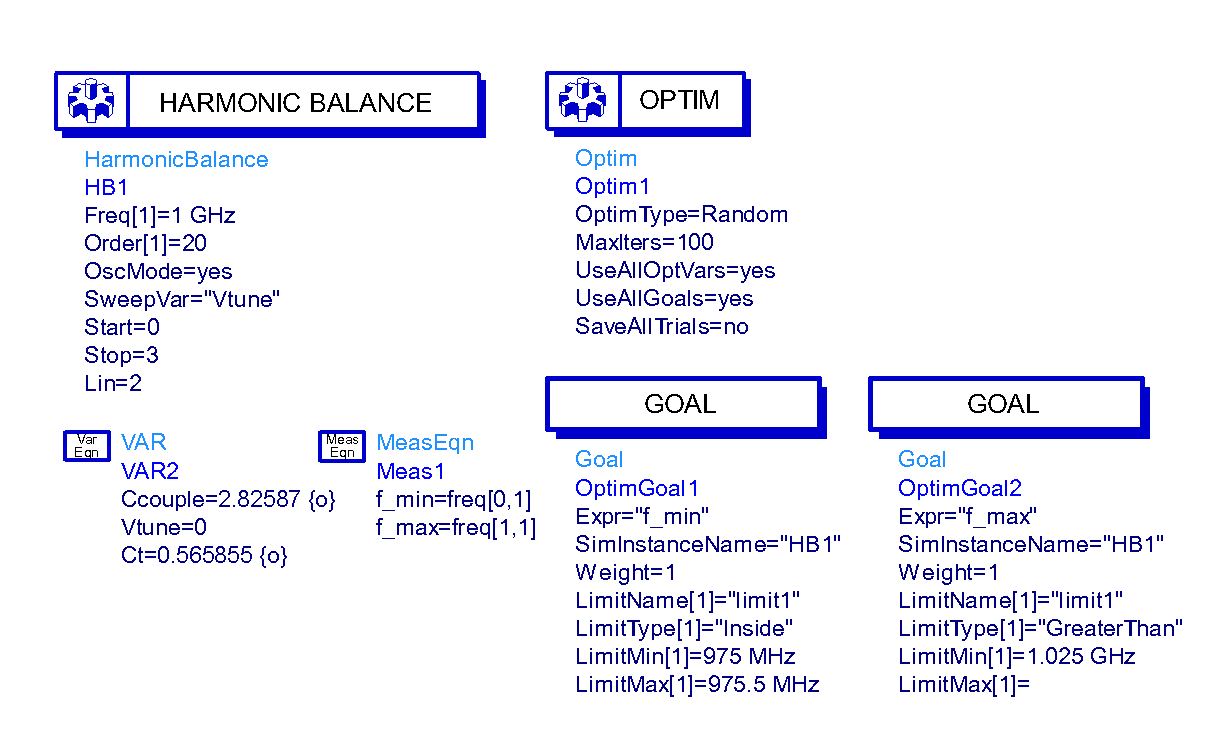
\includegraphics[width=0.8\textwidth]{Figures/3_VCO/vco_optimization_stage_controllers.pdf}
\caption{Configuración de los controladores de simulación y optimización en ADS.}
\label{fig:vco_optimization_controllers}
\end{figure}

Los resultados obtenidos fueron $C_{\text{couple}} = 2.82587$~pF y $C_t = 0.565855$~pF, adoptándose los valores comerciales de 2.9~pF y 0.55~pF para los análisis posteriores. En la Figura \ref{fig:vco_fosc_vtune} se puede observar el gráfico de $f_{\text{osc}}$ en función de la tensión de entrada $V_{\text{tune}}$.

\begin{figure}[htbp]
\centering
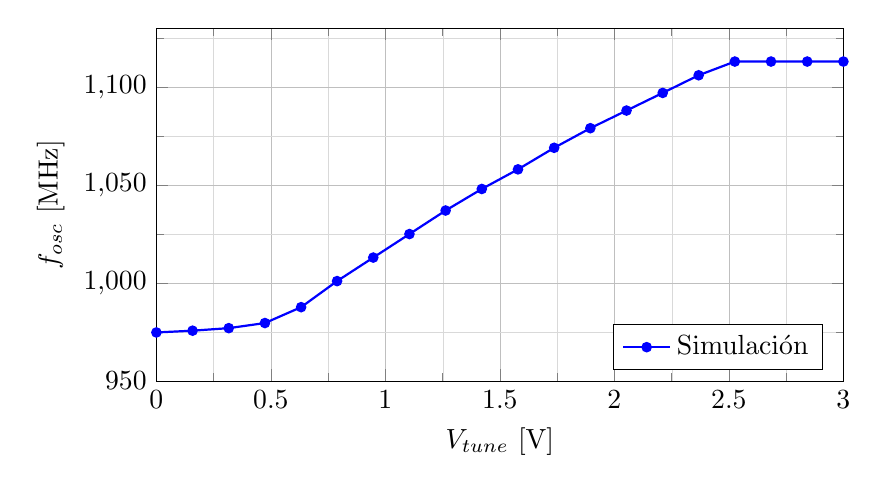
\begin{tikzpicture}
\begin{axis}[
    width=0.85\textwidth,
    height=0.5\textwidth,
    xlabel={$V_{\text{tune}}$ [V]},
    ylabel={$f_{\text{osc}}$ [MHz]},
    xmin=0, xmax=3,
    ymin=950, ymax=1130,
    grid=both,
    grid style={line width=.1pt, draw=gray!30},
    major grid style={line width=.2pt,draw=gray!50},
    minor tick num=1,
    legend pos=south east,
]
\addplot[
    color=blue,
    mark=*,
    mark size=1.5pt,
    thick,
] coordinates {
    (0.000, 974.8)
    (0.158, 975.7)
    (0.316, 977.0)
    (0.474, 979.6)
    (0.632, 987.7)
    (0.789, 1001.0)
    (0.947, 1013.0)
    (1.105, 1025.0)
    (1.263, 1037.0)
    (1.421, 1048.0)
    (1.579, 1058.0)
    (1.737, 1069.0)
    (1.895, 1079.0)
    (2.053, 1088.0)
    (2.211, 1097.0)
    (2.368, 1106.0)
    (2.526, 1113.0)
    (2.684, 1113.0)
    (2.842, 1113.0)
    (3.000, 1113.0)
};
\addlegendentry{Simulación}
\end{axis}
\end{tikzpicture}
\caption{Frecuencia de oscilación en función de la tensión de control $V_{\text{tune}}$.}
\label{fig:vco_fosc_vtune}
\end{figure}

De la curva se comprueba que para generar la señal chirp de 50~MHz (de 975~MHz a 1025~MHz) a la salida del VCO, se necesita una señal de diente de sierra a la entrada que varíe aproximadamente de 0.035~V a 1.105~V. Una linealización de la curva en la región activa (0.6~V a 2.5~V) propone la siguiente ecuación de transferencia:

\begin{equation}
f(V_{\text{tune}}) = 67.89 \cdot V_{\text{tune}} + 948.89 \quad [\text{MHz}]
\label{eq:vco_transfer}
\end{equation}

Se podría en una futura iteración del diseño ajustar el rango para que la variación de frecuencia quede en la zona lineal del varactor. También, el microcontrolador encargado de generar la señal diente de sierra podría teóricamente compensar los valores de la señal de control tal que a la salida se tenga una variación de frecuencia lineal.

\subsection{Análisis de Estabilidad}

Luego de obtener los valores correspondientes de los componentes, se procede a realizar un análisis de estabilidad utilizando la herramienta \texttt{OscTest} de ADS. Tomando como referencia el análisis realizado en el \textit{DesignGuide}, se obtiene el setup presentado en la Figura \ref{fig:vco_stability_analysis}. El análisis de estabilidad se realiza utilizando el criterio de Nyquist, donde la herramienta permite variar la impedancia de la sonda de prueba, manteniéndose en este caso en 50~$\Omega$.

\begin{figure}[htbp]
\centering
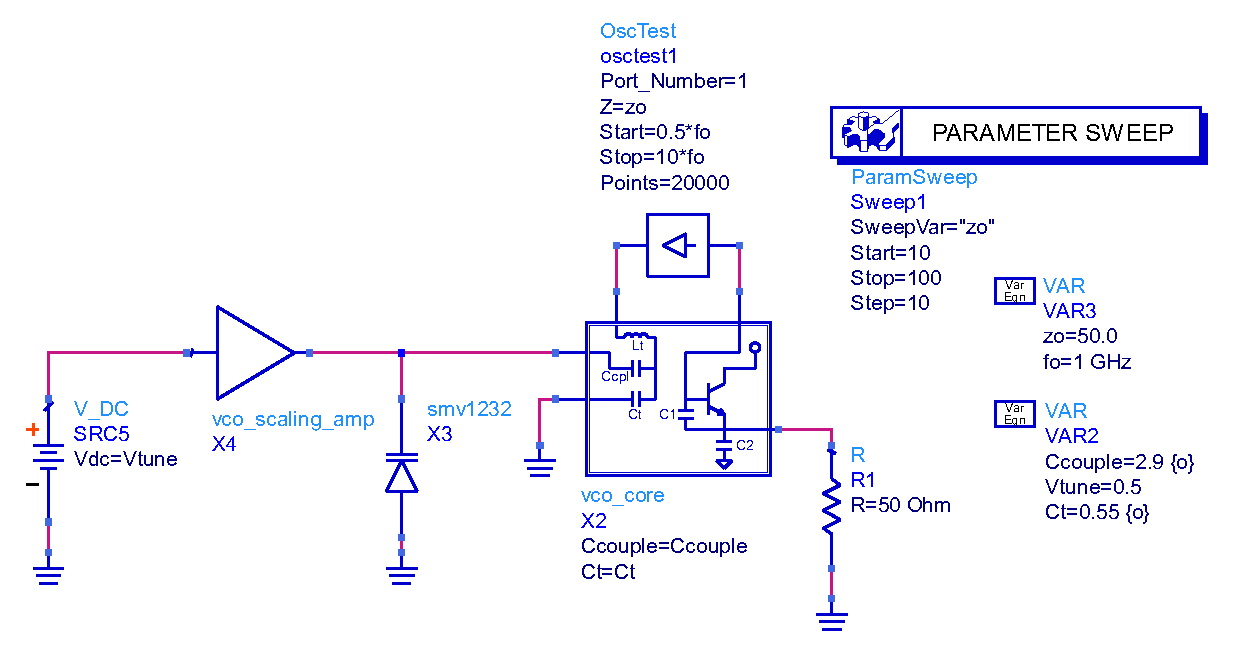
\includegraphics[width=0.95\textwidth]{Figures/3_VCO/vco_stability_analysis.pdf}
\caption{Configuración del análisis de estabilidad con \texttt{OscTest} en ADS.}
\label{fig:vco_stability_analysis}
\end{figure}

El criterio de Nyquist para osciladores basados en realimentación positiva establece que el circuito oscilará si la curva de $S_{11}$ en el plano polar rodea el punto $1 + j0$ en sentido horario. En la Figura \ref{fig:vco_stability_results} se presentan los resultados del análisis, donde se observa que efectivamente al variar la frecuencia se logra un lazo completo alrededor de $1 + j0$, condición requerida para la oscilación.

\begin{figure}[htbp]
\centering
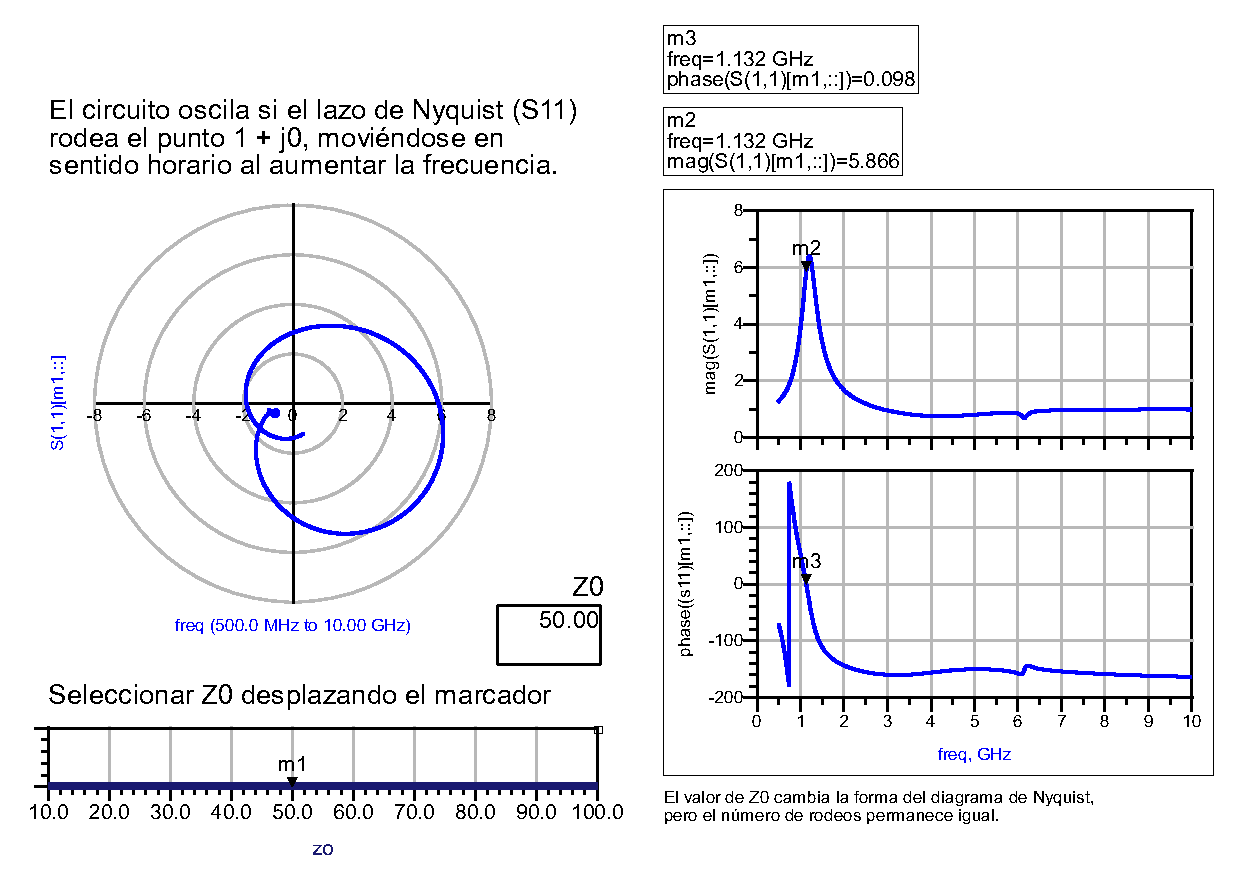
\includegraphics[width=0.95\textwidth]{Figures/3_VCO/vco_stability_analysis_results.pdf}
\caption{Resultados del análisis de estabilidad: diagrama de Nyquist y respuesta en frecuencia de $S_{11}$.}
\label{fig:vco_stability_results}
\end{figure}

La primera condición de arranque de oscilación requiere que la fase de $S_{11}$ sea de 0 grados a la frecuencia de oscilación. De los resultados se obtiene que a 1.132~GHz la fase es de aproximadamente 0.098 grados, cumpliendo esta condición. La segunda condición establece que la magnitud de $S_{11}$ debe ser mayor que 1; en este caso, la ganancia del lazo es de 5.866 (en veces), verificando así la condición de arranque.

Se puede concluir que el circuito oscilará correctamente y será capaz de sostener esta oscilación en el tiempo.

\subsection{Espectro de Salida y Potencia de la Señal}

Se procede a analizar el espectro resultante junto con el nivel de potencia de sus componentes. En la Figura \ref{fig:vco_power_analysis} se puede ver el setup propuesto para medir la potencia de salida, utilizando el nombre del nodo para realizar el análisis de oscilación.

\begin{figure}[htbp]
\centering
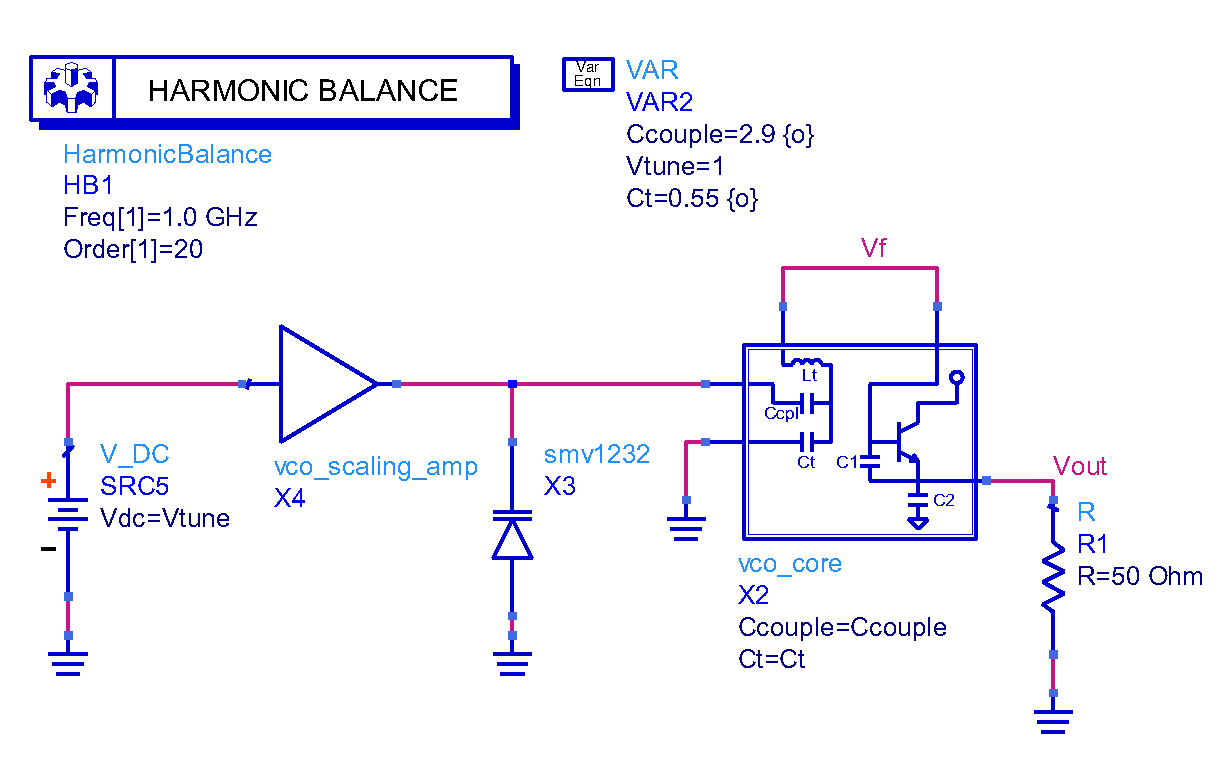
\includegraphics[width=0.95\textwidth]{Figures/3_VCO/vco_power_analysis.pdf}
\caption{Configuración para el análisis de potencia de salida del VCO.}
\label{fig:vco_power_analysis}
\end{figure}

En la Figura \ref{fig:vco_spectrum} se puede ver el resultado obtenido. Se obtuvo como componente fundamental $-0.635$~dBm en la frecuencia central de 1~GHz, lo cual es un nivel de potencia aceptable como entrada del amplificador de potencia. La segunda y tercera armónica tienen niveles de $-13.49$~dBm y $-26.29$~dBm respectivamente. La relación de potencia fundamental a segunda armónica es de 12.85~dBc, y a tercera armónica es de 25.65~dBc, valores aceptables para esta aplicación.

\begin{figure}[htbp]
\centering
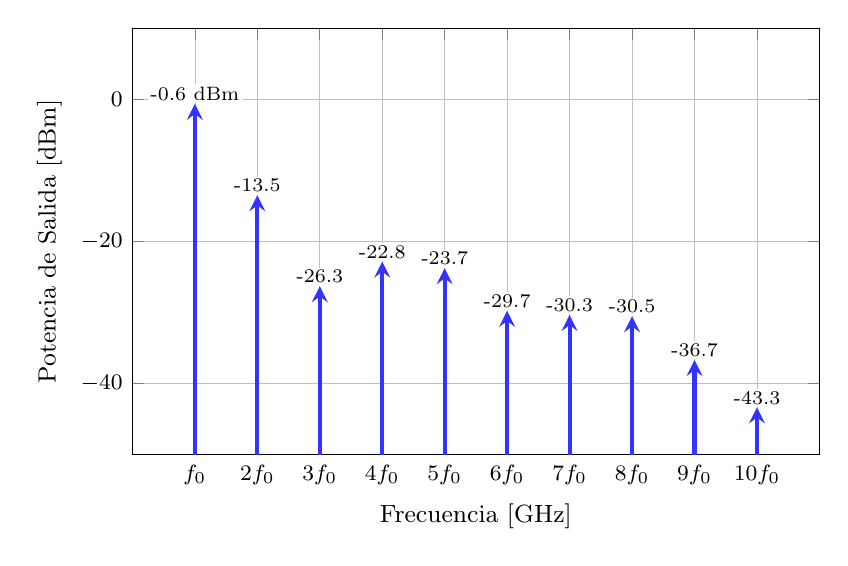
\begin{tikzpicture}
\begin{axis}[
    width=0.85\textwidth,
    height=7cm,
    xlabel={Frecuencia [GHz]},
    ylabel={Potencia de Salida [dBm]},
    xmin=0, xmax=11,
    ymin=-50, ymax=10,
    xtick={1,2,3,4,5,6,7,8,9,10},
    xticklabels={$f_0$, $2f_0$, $3f_0$, $4f_0$, $5f_0$, $6f_0$, $7f_0$, $8f_0$, $9f_0$, $10f_0$},
    grid=both,
    grid style={line width=.1pt, draw=gray!30},
    major grid style={line width=.2pt,draw=gray!50},
    tick label style={font=\footnotesize},
    label style={font=\small},
]
% Componentes espectrales como flechas desde el fondo
\draw[-stealth, blue!80, line width=1.5pt] (axis cs:1,-50) -- (axis cs:1,-0.64);
\draw[-stealth, blue!80, line width=1.5pt] (axis cs:2,-50) -- (axis cs:2,-13.49);
\draw[-stealth, blue!80, line width=1.5pt] (axis cs:3,-50) -- (axis cs:3,-26.29);
\draw[-stealth, blue!80, line width=1.5pt] (axis cs:4,-50) -- (axis cs:4,-22.82);
\draw[-stealth, blue!80, line width=1.5pt] (axis cs:5,-50) -- (axis cs:5,-23.75);
\draw[-stealth, blue!80, line width=1.5pt] (axis cs:6,-50) -- (axis cs:6,-29.75);
\draw[-stealth, blue!80, line width=1.5pt] (axis cs:7,-50) -- (axis cs:7,-30.33);
\draw[-stealth, blue!80, line width=1.5pt] (axis cs:8,-50) -- (axis cs:8,-30.51);
\draw[-stealth, blue!80, line width=1.5pt] (axis cs:9,-50) -- (axis cs:9,-36.66);
\draw[-stealth, blue!80, line width=1.5pt] (axis cs:10,-50) -- (axis cs:10,-43.32);

% Etiquetas de valores
\node[above, font=\scriptsize, fill=white, inner sep=1pt] at (axis cs:1,-0.64) {-0.6 dBm};
\node[above, font=\scriptsize, fill=white, inner sep=1pt] at (axis cs:2,-13.49) {-13.5};
\node[above, font=\scriptsize, fill=white, inner sep=1pt] at (axis cs:3,-26.29) {-26.3};
\node[above, font=\scriptsize, fill=white, inner sep=1pt] at (axis cs:4,-22.82) {-22.8};
\node[above, font=\scriptsize, fill=white, inner sep=1pt] at (axis cs:5,-23.75) {-23.7};
\node[above, font=\scriptsize, fill=white, inner sep=1pt] at (axis cs:6,-29.75) {-29.7};
\node[above, font=\scriptsize, fill=white, inner sep=1pt] at (axis cs:7,-30.33) {-30.3};
\node[above, font=\scriptsize, fill=white, inner sep=1pt] at (axis cs:8,-30.51) {-30.5};
\node[above, font=\scriptsize, fill=white, inner sep=1pt] at (axis cs:9,-36.66) {-36.7};
\node[above, font=\scriptsize, fill=white, inner sep=1pt] at (axis cs:10,-43.32) {-43.3};

\end{axis}
\end{tikzpicture}
\captionsetup{justification=centering}
\caption{Espectro de potencia de salida del VCO \\ mostrando la componente fundamental y sus armónicos.}
\label{fig:vco_spectrum}
\end{figure}

\subsection{Análisis de la Impedancia de Entrada del Núcleo}

Se analiza el valor complejo de impedancia de entrada del núcleo (\textit{core}) del oscilador. En la Figura \ref{fig:vco_impedance_analysis} se puede observar el setup utilizado para simular este parámetro, donde se conecta un puerto de prueba al nodo superior del circuito y se realiza un barrido de parámetros S desde 0.5~GHz hasta 3~GHz.

\begin{figure}[htbp]
\centering
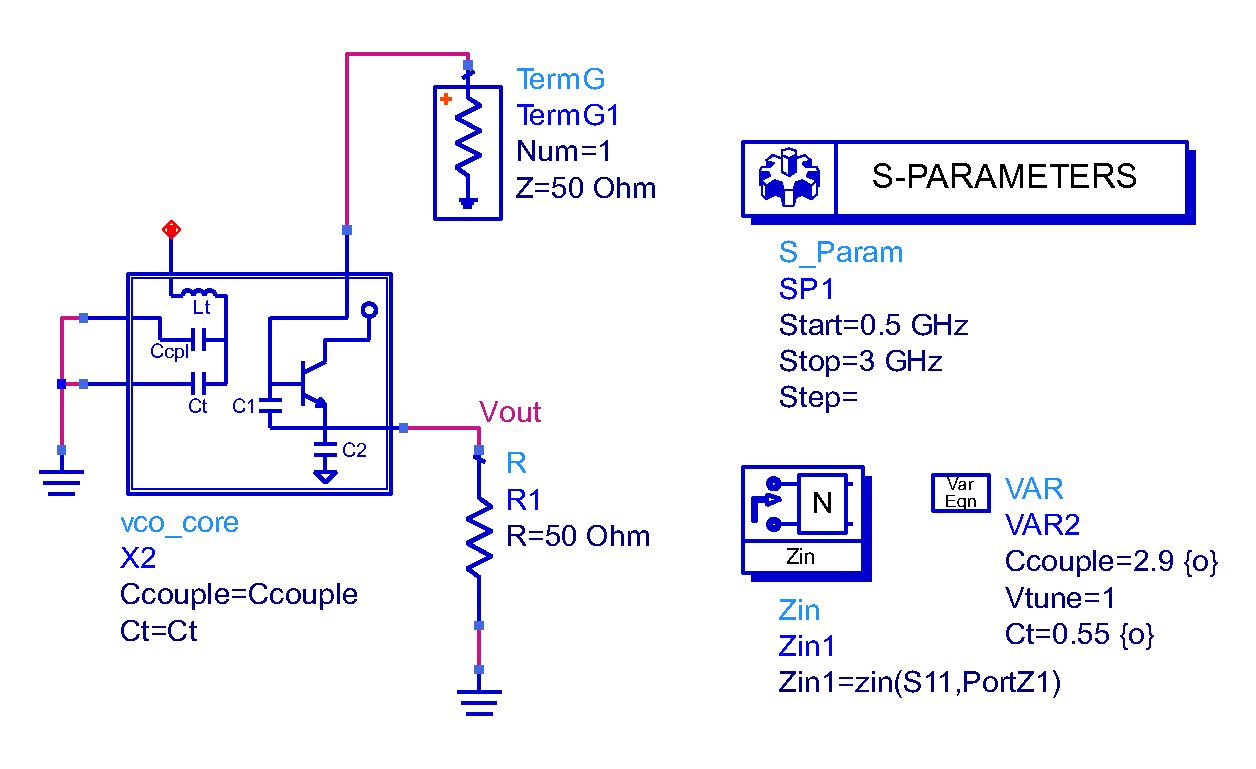
\includegraphics[width=0.85\textwidth]{Figures/3_VCO/vco_impedance_analysis.pdf}
\caption{Configuración para el análisis de impedancia de entrada del núcleo del oscilador.}
\label{fig:vco_impedance_analysis}
\end{figure}

En la Figura \ref{fig:vco_real_zin} se muestra la parte real de la impedancia de entrada del núcleo, mientras que en la Figura \ref{fig:vco_imag_zin} se muestra la parte imaginaria. Es importante notar que el componente real de la impedancia es negativo en todo el rango de frecuencia analizado; esto tiene sentido debido a que implica una resistencia negativa, que es un requerimiento fundamental en la condición de oscilación. Esta resistencia negativa suministra la energía que pierde el tanque LC del resonador debido a sus pérdidas parásitas.

\begin{figure}[htbp]
\centering
\begin{tikzpicture}
\begin{axis}[
    width=0.9\textwidth,
    height=7cm,
    xlabel={Frecuencia [GHz]},
    ylabel={$\text{Re}(Z_{\text{in}})$ [$\Omega$]},
    xmin=0.5, xmax=3,
    ymin=-300, ymax=0,
    grid=both,
    grid style={line width=.1pt, draw=gray!30},
    major grid style={line width=.2pt,draw=gray!50},
    tick label style={font=\footnotesize},
    label style={font=\small},
]
\addplot[red, thick] table[
    x expr=\thisrowno{0}/1e9,
    y expr=\thisrowno{1},
    col sep=tab,
    skip first n=1
] {Datasets/3_VCO/data_vco_real_zin.dat};

% Marcador a 1 GHz
\addplot[only marks, mark=*, mark size=3pt, red] coordinates {(1.005, -69.01)};
\node[anchor=south west, font=\scriptsize, fill=white, inner sep=2pt] at (axis cs:1.05,-85.01) {$-69.0\ \Omega$ @ 1.005 GHz};

\end{axis}
\end{tikzpicture}
\caption{Parte real de la impedancia de entrada del núcleo del oscilador.}
\label{fig:vco_real_zin}
\end{figure}

A la frecuencia de interés (aproximadamente 1~GHz), la parte real de la impedancia es de $-69.0\ \Omega$. Este valor de resistencia negativa es robusto y significa que el oscilador podrá arrancar incluso si el tanque LC tiene pérdidas resistivas de hasta $69\ \Omega$. En diseño práctico se busca que $|R_{\text{neg}}|$ sea 2 o 3 veces mayor que la resistencia de carga para asegurar un arranque rápido y confiable.

\begin{figure}[htbp]
\centering
\begin{tikzpicture}
\begin{axis}[
    width=0.9\textwidth,
    height=7cm,
    xlabel={Frecuencia [GHz]},
    ylabel={$\text{Im}(Z_{\text{in}})$ [$\Omega$]},
    xmin=0.5, xmax=3,
    ymin=-180, ymax=20,
    grid=both,
    grid style={line width=.1pt, draw=gray!30},
    major grid style={line width=.2pt,draw=gray!50},
    tick label style={font=\footnotesize},
    label style={font=\small},
]
\addplot[blue, thick] table[
    x expr=\thisrowno{0}/1e9,
    y expr=\thisrowno{1},
    col sep=tab,
    skip first n=1
] {Datasets/3_VCO/data_vco_imag_zin.dat};

% Marcador a 1 GHz
\addplot[only marks, mark=*, mark size=3pt, blue] coordinates {(1.005, -23.40)};
\node[anchor=south west, font=\scriptsize, fill=white, inner sep=2pt] at (axis cs:1.05,-35.40) {$-23.4\ \Omega$ @ 1.005 GHz};

\end{axis}
\end{tikzpicture}
\caption{Parte imaginaria de la impedancia de entrada del núcleo del oscilador.}
\label{fig:vco_imag_zin}
\end{figure}

La parte imaginaria a 1.005~GHz es de $-23.4\ \Omega$, lo que indica que el núcleo del oscilador tiene un comportamiento capacitivo a esta frecuencia. Para que el circuito resuene, el tanque resonante externo debe presentar una reactancia inductiva que cancele esta capacitancia, cumpliendo la condición de resonancia $\text{Im}(Z_{\text{total}}) = 0$.

En resumen, a la frecuencia de operación de 1~GHz, el núcleo presenta una impedancia de entrada de $Z_{\text{in}} = -69.0 - j23.4\ \Omega$, confirmando que el circuito está correctamente polarizado y genera suficiente resistencia negativa para sostener las oscilaciones.

\subsection{Período Transitorio y Estado Estacionario en el Dominio del Tiempo}

Se analiza el transitorio y el estado del sistema luego del mismo, en el dominio del tiempo. En la Figura \ref{fig:vco_transient_analysis} se presenta el esquemático de la simulación, donde se configuran dos análisis transitorios: uno de 0 a 50~ns para observar el arranque, y otro de 990~ns a 1000~ns para verificar el estado estacionario.

\begin{figure}[htbp]
\centering
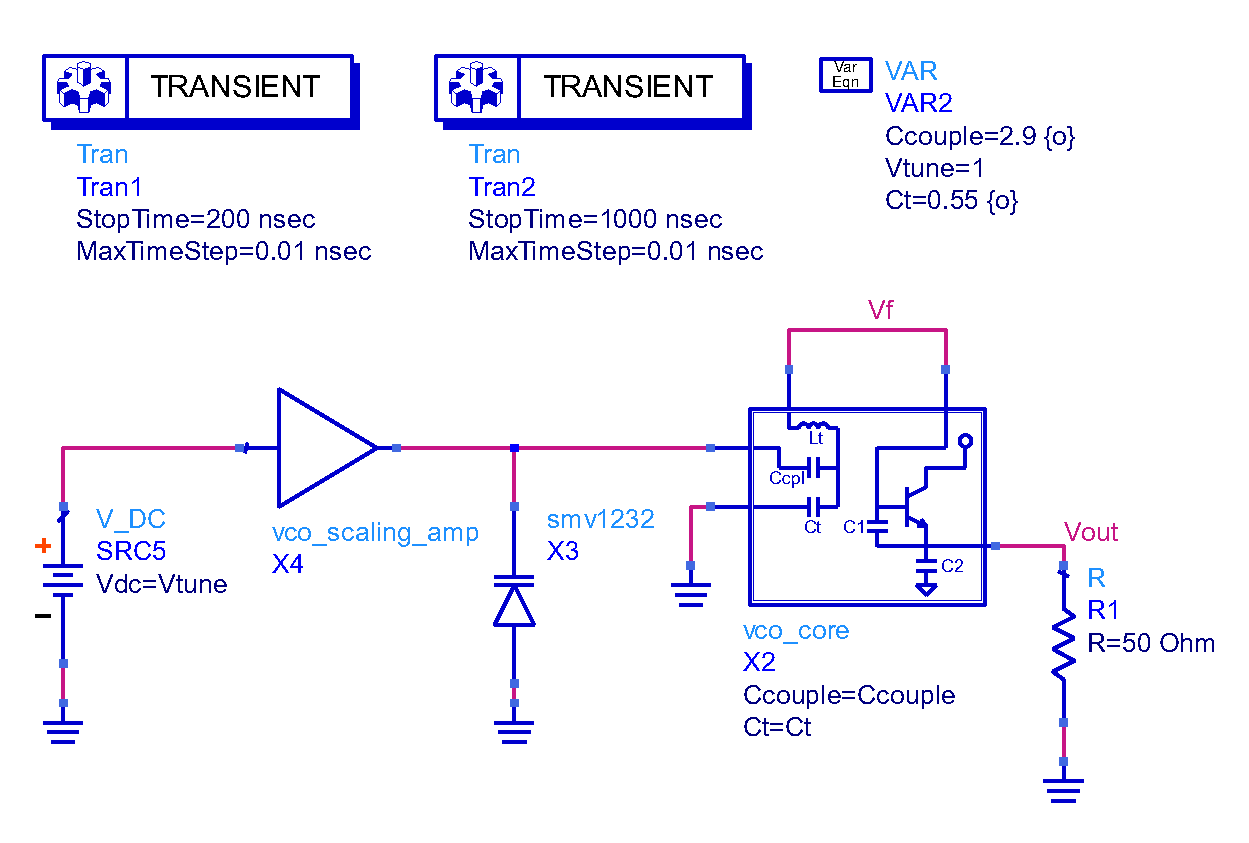
\includegraphics[width=0.95\textwidth]{Figures/3_VCO/vco_transient_analysis.pdf}
\caption{Configuración para el análisis transitorio del VCO.}
\label{fig:vco_transient_analysis}
\end{figure}

En la Figura \ref{fig:vco_startup} se observa el período transitorio del oscilador. Durante los primeros 20~ns aproximadamente, el oscilador amplifica únicamente ruido térmico con amplitud infinitesimal. Entre 20~ns y 30~ns se produce un crecimiento exponencial de la oscilación, confirmando que la condición $|R_{\text{neg}}| > R_{\text{pérdidas}}$ se cumple correctamente. A partir de los 30~ns, la amplitud comienza a saturarse debido a las no linealidades del transistor. Se puede observar que el sistema alcanza el estado estacionario luego de aproximadamente 40 a 50~ns.

\begin{figure}[htbp]
\centering
\begin{tikzpicture}
\begin{axis}[
    width=0.95\textwidth,
    height=7cm,
    xlabel={Tiempo [ns]},
    ylabel={$V_{\text{out}}$ [V]},
    xmin=0, xmax=50,
    ymin=-0.5, ymax=0.4,
    grid=both,
    grid style={line width=.1pt, draw=gray!30},
    major grid style={line width=.2pt,draw=gray!50},
    tick label style={font=\footnotesize},
    label style={font=\small},
]
\addplot[red, thick, each nth point=1] table[
    x expr=\thisrowno{0}*1e9,
    y expr=\thisrowno{1},
    col sep=tab,
    skip first n=1
] {Datasets/3_VCO/data_vco_tran_0_50_ns_reduced.dat};
\end{axis}
\end{tikzpicture}
\caption{Período transitorio del oscilador (arranque).}
\label{fig:vco_startup}
\end{figure}

En la Figura \ref{fig:vco_steady_state} se observa el estado estacionario del sistema. Si bien el período coincide con el de una señal de 1~GHz (aproximadamente 10 ciclos en 10~ns), se nota una deformación en la señal: las crestas superiores son más redondeadas mientras que los picos inferiores son más agudos. Este es un comportamiento esperado en este tipo de osciladores de gran señal (\textit{Large Signal}). La tensión de salida varía aproximadamente de $-410$~mV a $+280$~mV, resultando en una amplitud pico a pico de aproximadamente 690~mV.

\begin{figure}[htbp]
\centering
\begin{tikzpicture}
\begin{axis}[
    width=0.95\textwidth,
    height=7cm,
    xlabel={Tiempo [ns]},
    ylabel={$V_{\text{out}}$ [V]},
    xmin=990, xmax=1000,
    ymin=-0.5, ymax=0.4,
    grid=both,
    grid style={line width=.1pt, draw=gray!30},
    major grid style={line width=.2pt,draw=gray!50},
    tick label style={font=\footnotesize},
    label style={font=\small},
]
\addplot[red, thick, each nth point=1] table[
    x expr=\thisrowno{0}*1e9,
    y expr=\thisrowno{1},
    col sep=tab,
    skip first n=1
] {Datasets/3_VCO/data_vco_tran_990_1000_ns_reduced.dat};
\end{axis}
\end{tikzpicture}
\caption{Estado estacionario del oscilador.}
\label{fig:vco_steady_state}
\end{figure}

\section{Conclusiones}

Se diseñó y simuló exitosamente un Oscilador Controlado por Tensión basado en la topología Clapp modificada en configuración colector común, operando a una frecuencia central de 1~GHz. El VCO cumple con los requerimientos establecidos: presenta un rango de sintonía de 50~MHz controlado mediante una tensión de entrada que varía de 0~V a 1.1~V, entrega una potencia de salida de $-0.6$~dBm en la componente fundamental, y demuestra un arranque robusto en aproximadamente 40~ns. Los análisis de estabilidad confirman que el circuito genera suficiente resistencia negativa para sostener las oscilaciones, y las simulaciones en el dominio del tiempo verifican el correcto funcionamiento del oscilador en estado estacionario.
